% 2010 年湖北卷理科第 7 题：半径 r 的圆、内接正六边形、其内切圆及再内接正六边形。
% 来源 PDF：普通高考/2010/2010湖北理.pdf，SHA-256 2cfb3d100d55f89c58fe4475caf29f039496afbd0f16d7a7d07857eed5759f55。
% 原页：第 1 页（A3 三栏）第 2 栏顶部，书页码 597。
% 重绘依据：按 600 dpi 原页量得外圆半径 r 与内切圆半径之比为 1:(√3/2)；
%   两个正六边形取向相同，均有水平的上、下边（顶点位于 0°,60°,…,300°），
%   虚线 r 由圆心 O 连到外六边形位于 120° 的顶点（即外圆上的点）。
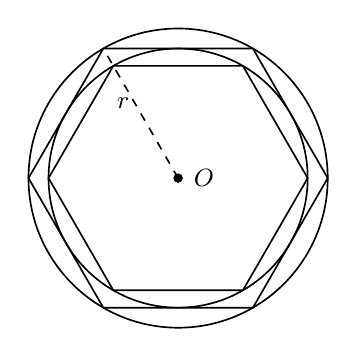
\begin{tikzpicture}[scale=1.9, semithick, every node/.style={inner sep=1.6pt, font=\small}]
  % 外圆与内切圆
  \draw (0,0) circle (1);
  \draw (0,0) circle (0.8660254);
  % 外接正六边形（外圆半径 1）
  \draw (0:1) \foreach \a in {60,120,180,240,300,360} { -- (\a:1) };
  % 内接正六边形（内切圆半径 √3/2）
  \draw (0:0.8660254) \foreach \a in {60,120,180,240,300,360} { -- (\a:0.8660254) };
  % 半径 r
  \draw[dashed] (0,0) -- (120:1);
  \node[left] at (120:0.58) {$r$};
  \fill (0,0) circle (0.9pt);
  \node[right] at (0.07,0) {$O$};
\end{tikzpicture}
